\documentclass[conference,10pt]{IEEEtran}

\usepackage{hyperref}
\usepackage{graphicx}

\ifCLASSOPTIONcompsoc
    \usepackage[caption=false, font=normalsize, labelfont=sf, textfont=sf]{subfig}
\else
    \usepackage[caption=false, font=footnotesize]{subfig}
\fi
\captionsetup[subfigure]{width=0.48\textwidth} % 讓 caption 最大寬度一致

\title{03\_1 Figure IEEEtran}
\author{Po-Hsuan Huang\\ 
    \texttt{aben20807@gmail.com}
}

\begin{document}
\vspace*{-50pt}
    {\let\newpage\relax\maketitle}

\section{subfig}

Test reference: Figure~\ref{fig:all}, \ref{fig:example}, and \ref{fig:cat}.

\begin{figure}[htb!]
    \centering
    \subfloat[Caption for example.]{\label{fig:example}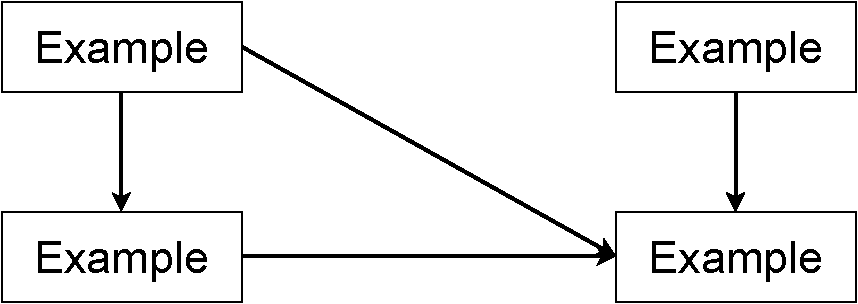
\includegraphics[width=0.33\textwidth]{figures/paper-example.pdf}}\hfill%
    \subfloat[\tiny Cat.]{\label{fig:cat}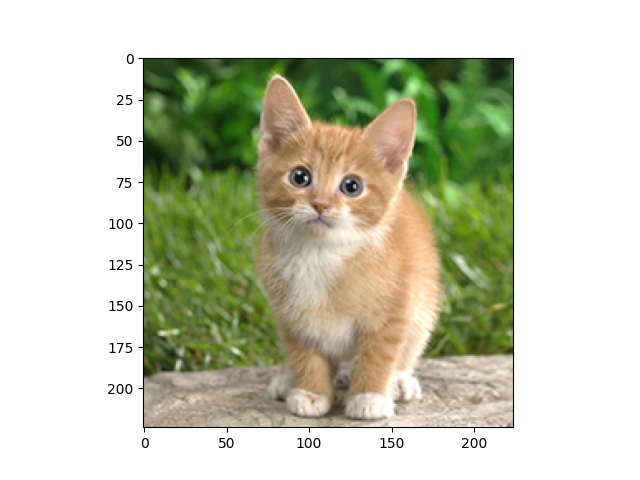
\includegraphics[width=0.48\textwidth]{figures/cat.png}}%
    \caption{Two subfigures.}
    \label{fig:all}
  \end{figure}

\end{document}